\documentclass[11pt, oneside]{article}   	% use "amsart" instead of "article" for AMSLaTeX format
\usepackage{geometry}                		% See geometry.pdf to learn the layout options. There are lots.
\geometry{letterpaper}                   		% ... or a4paper or a5paper or ... 
%\geometry{landscape}                		% Activate for for rotated page geometry
%\usepackage[parfill]{parskip}    		% Activate to begin paragraphs with an empty line rather than an indent
\usepackage{graphicx}				% Use pdf, png, jpg, or eps§ with pdflatex; use eps in DVI mode
								% TeX will automatically convert eps --> pdf in pdflatex		
\usepackage{amssymb}
\usepackage{amsmath}
\usepackage{setspace}
\usepackage[square,sort,comma,numbers]{natbib} \bibpunct{(}{)}{;}{author-year}{}{,} 
\usepackage[hidelinks]{hyperref}


\title{Local PCA Shows How Population Structure Differs Along the Genome}
\author{Han Li, Peter Ralph}
%\date{}							% Activate to display a given date or no date

\usepackage{color}
\newcommand{\plr}[1]{{\em \color{blue} #1}}


\begin{document}
\maketitle
%\section{}
%\subsection{}
\doublespacing


\section*{Abstract}

Dimension reduction techniques,
such as principal components,
are often used to discover and display large-scale structure in genomic datasets
found in the patterns of kinship
between the genotyped individuals,
and to control for the confounding effects of population structure in genome-wide association studies.
The genome-wide mean kinship this uses
is an average of the relationships across all locus-specific genealogical trees.
However, many biological factors,
including linked selection,
can systematically skew patterns of kinship over intermediate genomic scales.
We show how to use principal components analysis (PCA) to describe this meso-scale variation in kinship,
and apply the method to genomic data from three species.
In each species we find substantial variation on the scale of megabases to tens of megabases.
In a global human dataset, small, discontinuous variation is likely explained by polymorphic chromosomal inversions.
In a dataset of African \textit{Drosophila melanogaster}, large, continuous variation across each chromosome arm
is explained by known chromosomal inversions thought to be under recent selection.
In a range-wide dataset of \textit{Medicago truncatula},
common axes of variation in population structure are shared between chromosomes,
correlate with local gene density,
and may be caused by background selection or local adaptation.
The method is a useful addition to the exploratory toolbox
of population genomics.

\plr{Add percent of variance explained by first two MDS coordinates, after subtracting the genome-wide mean covariance matrix.}

\plr{Add whole-genome PCA plots for comparison (unless they look just like one of the three corners; in which case say so.}

\section{Introduction}

% The kinship matrix contains the kinship coefficient for pairwise individuals. 
% Kinship coefficient defines the genetic relatedness between individuals.
% It is the probability that two alleles randomly selected from two individuals are inherited from the most recent common ancester.
% It could be estimated from given pedigree or from genome-wide covariances of genotype markers. 
% It is well-known that for kinship matrix, actual relatednesses have a lot of noise about the expected value, and depend on where on the genome you look; this is why scans for selective sweeps work.
% Populations are often structured in some way while there are systematic genetic variation between populations. 


The phrase ``population structure'' refers to reduced gene flow between subpopulations, 
often because of geographical isolation.
However, it is widely recognized that because of selection the effects of gene flow are not equal everywhere on the genome,
and patterns of polymorphism and divergence can vary significantly depending on factors including local gene density.
This implies that, paradoxically, 
the population structure of a species depends on which part of the genome is being examined.

Population structure leads to systematic patterns in genome-wide mean kinship,
and so it is said that visualizations of kinship depict population structure,
rather than the \emph{effects} of population structure (which would be more accurate).
The \emph{kinship coefficient} for a pair of individuals
gives the expected proportion of their genome
that the two have inherited identically by descent;
for a single individual it is the inbreeding coefficient.
However, as \citet{wright1949genetical} wrote,
``It has probably occurred to the reader that the coefficient of inbreeding
may mean very different things in different cases.''
The kinship coefficient originally referred to the expected probability
of coinheritance within a given pedigree;
while modern applications to ``unrelated'' individuals
use a genetic covariance matrix to estimate the \emph{realized} proportion of the genome
coinherited from sufficiently recent ancestors.

Realized kinship summarizes the shapes
of the genealogical that relate the samples
at each location along the genome.
Since these trees vary along the genome, so does realized kinship;
but averaging over sufficiently many trees we hope to get a stable estimate,
independent of the genomic region chosen.
This hope is not entirely justified: for instance,
kinship on sex chromosomes is expected to differ from the autosomes;
and positive or negative selection on particular loci can dramatically disort shapes of nearby genealogies
\citep{maynardsmith1974hitchhiking,barton2000genetic,neher2013genetic,charlesworth2012effects},
and therefore patterns of kinship.
Indeed,
chromosome-scale variation in diversity and divergence has been observed in many species
\citep[e.g.][]{sattath2011pervasive};
species phylogenies can differ along the genome 
due to incomplete lineage sorting \citep[e.g.][]{pease2013accurate},
adaptive introgression and/or local adaptation \citep[e.g.][]{ellegren2012genomic,nadeau2012genomic,pool2015natural,vernot2014resurrecting};
and theoretical expectations predict that geographic patterns of relatedness should depend on selection
\citet{charlesworth2003review}.
Nonetheless, it is not generally known to what extent patterns of kinship vary along the genome,
nor what the major axes of variation are.


Patterns in genome-wide kinship are often summarized
by applying principal components analysis (PCA) \citep{patterson2006population} 
to the genetic covariance matrix,
as pioneered by \citet{menozzi1978synthetic}.
% About 37 years ago, \citet{menozzi1978synthetic} first applied principal component analysis (PCA) in population genetics to construct maps summarizing genetic variation \citep{menozzi1978synthetic}. 
% Nowadays, PCA is a widely used powerful non-parametric method to extract information from genetic data.  
% PCA results are derived from the covariance matrix of genotype matrix. 
The results of PCA can be directly related to the underlying genealogical history of the samples, 
such as time to most recent common ancestor and migration rate between populations \citep{novembre2008interpreting,mcvean2009genealogical}. 
These patterns are often geographical, producing ``maps'' of population structure
that reflect the samples' geographic origin distorted by rates of gene flow
\citep{novembre2008genes},
although other patterns emerge if recent migration or nongeographic kinship patterns are important
\citep{astle2009population}.
% Through dimension-reduction, PCA can identify key components of population structure, which describes how different samples are related, and are often closely related to geography. 
% Plots of the first two principal components (PCs) can mimic the samples' geographic origin to some extent. 
% Since population structure describes how different samples are related, samples living closer tend to be more genetically similar and thus tend to be clustered in PC plots \citep{novembre2008genes,patterson2006population}. 
% However this relatedness is limited while there's recent migration or for group with nongeographic kinship patterns,for example, social or religious groups. \citep{astle2009population}

As reviewed by \citet{astle2009population}, 
modeling ``background'' kinship between samples
is essential to successful genome-wide association studies,
and PCA has often been used for stratification correction \citep{price2006principal},
and so investigating variation in kinship along the genome can help us to have a
better understanding of the relation between genome structure 
and population structure, possibly leading to more powerful methods for association studies.

To investigate how population structure varies along the genome in several datasets, 
we cut each genome into windows (with hundreds to thousands of SNPs in each), 
applied PCA to each window, 
and visualized the major ways that population structure, as summarized by PCA, varies among windows.
% In this project, we used SNP data for human, \textit{Medicago truncatula}, and
whole genome sequencing data for \textit{Drosophila}.  
% Based on the principal components, we can estimate the similarity of population structure contained in each genome window.  
To quantify similarity of population structure between
windows, we constructed for each window an approximate, scaled covariance
matrix based on the first few principal components, and measured the pairwise Euclidean distance
between those matrices.  
We then use multidimensional scaling to visualize the
relationships between windows, which reduces the pairwise distance matrix to
lower dimension while preserving the distance information between windows as
well as possible \citep{borg2005modern}.  

% To interpret the results of MDS, we combine known genome feature information for each species, such as the
% distribution of inversions, and heterochromatin and gene density along the genome. 
Each species showed distinct patterns, reflecting differences in their biology;
before presenting results,
it may help to have a prior idea of what factors are expected to affect population structure,
and how.
PCA summarizes patterns in kinship found in the genetic covariance matrix,
which is an average across locus-specific genealogies.
% However, different parts of genome have different genetic features. 
% First, each site of DNA may have different gene tree. 
% The covariance matrix of genotype matrix averages those gene trees. 
If individuals are closer in the genealogies of a given genomic region, 
they tends to be more close in the PCA maps for that region. 
% Different DNA segments may have different gene tree and therefore different population structure for those segments. 
% Second, the strength of linked selection differs for different DNA segments, and produces different population structure in region under linked selection compared to other region. 
% Selective sweeps cause local recent ancestry or short trees.
% Background selection causes shallow ones.
Strong selective sweeps of beneficial alleles can lead to relatively long genomic regions
characterized by short genealogical trees \citep{przeworski2005signature,garud2013selective}.
A genomic region with many targets for selection experiences
background selection and/or recurrent selective sweeps \citep{stephan1992effect,coop2012patterns},
which would tend to generally shorten genealogical trees in the region,
similar to a reduction in effective population size \citep{hudson1995deleterious}.
% Balancing selection causes deep trees.
On the other hand, balancing selection leads to very deep trees \citep{gao2014footprints},
and population structure locally describes which individuals have which alleles
rather than geographical proximity.
Finally, 
since recombination is suppressed between opposite orientations of a chromosomal inversion
near its breakpoints,
genealogies in these regions separate samples carrying the two orientations of the inversion.
In the resulting extended block, population structure shows two (for haploids) or three (for diploids) clusters
(indeed, \citep{ma2012investigation} has proposed using trimodality of local PCA plots
as a way to identify inversions).
% if a chromosomal inversion is polymorphic in the sample, 
% the regions around the breakpoints of inversions usually have high linkage disequilibrium and the two directions of a inversion will have different linked alleles around the breakpoints. Recombination suppression across inversions thus results in different genome structure and population structure. 
% Other effects, like noise, introgression might also influence population structure.
We will look for strong variation in population structure shared across large regions of the genome.
Many of the effects listed above (such as single selective sweeps or inversions) 
are not expected to have similar effects on population structure in different regions of the genome
because of randomness in which samples end up in which group;
but if these coincide with a region of reduced recombination (such as an inversion),
these could drive major patterns of variation.
The more subtle effects of genome-wide linked selection could be shared across large regions
due to large-scale variation in gene density
(as by background selection or local adaptation at many genes).


We chose PCA to summarize population structure,
but other methods, such as STRUCTURE \citep{falush2003inference},
SPA \citep{yang2012modelbased},
SpaceMix \citep{bradburd2015spatial},
or other matrix factorization methods \citep{engelhardt2010analysis}
would highlight different sources of variation in the data.
% There are other methods for visualizing population structure are like STRUCTURE,
% \citep{pritchard2000inference,falush2003inference, falush2007inference,hubisz2009inferring} 
% model-based approach,
% maps of heterozygosity
% \citep{ramachandran2005support}. 

Finally, a number of general methods for dimensionality reduction also use a strategy of ``local PCA''
\citep[e.g.][]{manjon2013diffusion,kambhatla1997dimension,weingessel2000local,roweis2000nonlinear},
performing PCA not on the entire dataset but instead on subsets of observations,
providing ``local'' pictures which are then stitched back together to give a global picture.
At first sight,
this differs from our use of the term in that we restrict to subsets of \emph{variables} instead of subsets of observations.
However, if we flip perspectives and think of each genetic variant as an observation,
our method shares common threads, although the ultimate goals and methods for visualization are different.
Future methods for visualization of genomic data
may benefit from other advances in this substantial literature 
\citep[reviewed in][]{vandermaaten2009dimensionality}.



\section{Methods}

\plr{How about: first describe the method; then afterwards, present the three datasets.}
\begin{figure}
    \begin{center}
       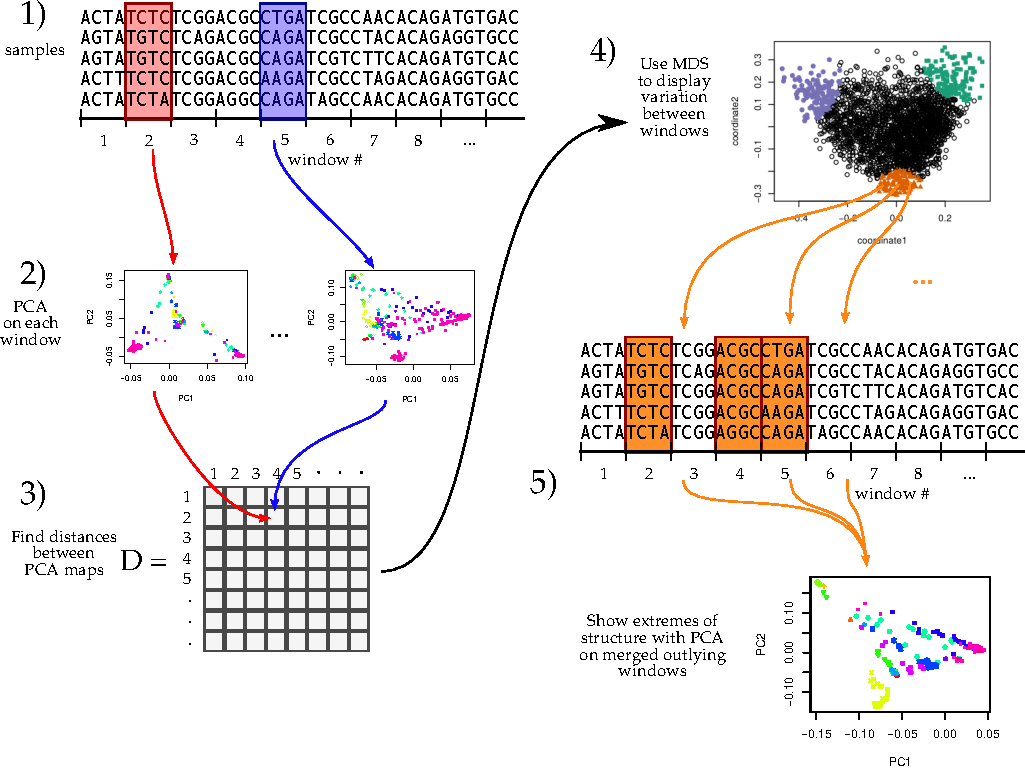
\includegraphics[width=0.9\textwidth]{the-method-diagram}
    \end{center}
    \caption{
         The diagram of our method.
         \label{fig:diagram}
    }
\end{figure}



\subsection{Recode the DNA sequence to a matrix consisting of 0,1,2 (and NA).}

For human, we use SNP chip data from POPRES \citep{nelson2008population}. There are 3,965 samples in total, (346 African-Americas; 73 Asians; 3,187 Europeans; 359 Indian Asians), and the 22 autosomes together have 447,267 SNPs in this dataset. 
We use the allele that has highest frequency in the samples as the reference allele for each position. 
The first step is to recode genetic data as a numeric matrix; 
which we take to have one row per variant and one column per sample. (omitting monomorphic variants)
In our applications, for each variant we picked a reference allele, 
and recoded genotypes as the number of non-reference alleles carried by the individual;
obtaining 0,1, or 2 for autosomal variants in diploids, or NA for missing data.
A normalization step (see below) ensures the result does not depend on the choice of reference allele.

For \textit{Drosophila melanogaster}, we use the sequencing data from Drosophila Population Genomics Project (DPGP) and John Pool's lab \citep{lack2015drosophila}, 
which together has 380 samples from 16 countries across Africa and Europe.
Each chromosome arm we investigated (Chr2L, Chr2R, Chr3L, Chr3R) has 2-3 million SNPs.
Due to high density of missing data for some parts in the genome, we then delete the samples with more than 8\% missing genotypes and then deleting positions with more than 20\% missing data. 
The cutoff points 8\% and 20\% are determined from the corresponding distributions of NAs in samples and at positions. 
Since the \textit{Drosophila} samples are from inbred lines with little heterozygosity, we treat the samples as haploid when recoding.

For \textit{Medicago truncatula}, we use the SNP data from whole genome sequencing from \textit{Medicago truncatula} Hapmap Project \citep{tang2014improved}. 
It has 263 samples from 24 countries. 
Each of the 8 chromosomes has 3-5 million SNPs.

\begin{table}[ht]
\centering
\begin{tabular}{p{0.8in}p{1in}p{1in}p{1in}p{1.2in}}
  \hline
 & species number of SNPs per window & mean length in bp per window & mean number of windows per chromosome & mean ratio of variance explained by top 2 PCs \\ 
  \hline
\textit{Drosophila melanogaster} & 1000 & 9019 & 2674 & 0.53 \\ 
  Human & 100 & 636494 & 203 & 0.55 \\ 
  \textit{Medicago truncatula} & 10000 & 102580 & 467 & 0.50 \\ 
   \hline
\end{tabular}
\caption {some statistic for each species' genome}
\end{table}


\subsection{PCA in genomic windows}

After recoding, we divided the recoded matrix into contigous matrixes that have the same columns but fewer rows than the original matrix, 
and applied Principal Component Analysis (PCA) separately on each window, 
following the procedure in \citet{mcvean2009genealogical} as follows. Starting with the recoded genotype matrix $Z$, 
where $Z$ is a $L\times N$ matrix ( $L$ is SNP number ; $N$ is sample size), 
first compute the mean-centered matrix $X$, $X_{si}=Z_{si}-\overline{Z_{s}}$, 
where $\overline{Z_{s}}$ is the mean of non-missing entries, $\overline{Z_{s}}=\frac{1}{n}\sum_{j=1}^{n}Z_{sj}$.
The mean-centering step makes the result not depend on the choice of reference allele.
Then find the covariance matrix of $X$, denoted $C=\frac{1}{n-1}XX^{T}$. 
We compute the covariance matrix using the R function cov() , with use=``pairwise",
which computes the covariance between each pair of individuals using all complete pairs of SNPs on those individuals.
The principal components are eigenvector of C, ordered by magnitude of the eigenvalues.

The top few principal components generally display population structure; we usually use the first two (referred to as PC1 and PC2).

\subsubsection{Choosing window length}
The window length should neither be too long or too short. 
In general, longer windows have more SNPs, 
the noise (the mean standard error within a window) will be smaller
and so population structure in that window will be more accurately estimated.
However, to better resolve features along the genome, we need reasonably short windows 
to have stronger signal (the mean standard variation between windows).
If we use the first principal component as a measure of population structure, 
then to choose a proper length for a window, 
we need to find a balance between variance of the first principal components inside a window and that between windows. 
The variance between windows is estimated by the mean variance of the first principal component for each window. 
$Var_{between}= \frac{1}{N}\sum_{j=1}^{N}\left ( \frac{1}{K}\sum_{i=1}^{K}\left ( PC1_{i,j} -\overline{PC1_{,j}} \right )^{2} \right )$ ($K$ is the number of windows on the genome)
The variance inside a window is estimated using the block jackknife cutting the window into 10 equal size smaller windows \citep{efron1982jackknife}. 
$Var_{inside}= \frac{1}{N}\sum_{j=1}^{N}\left ( \frac{9}{10}\sum_{i=1}^{10}\left ( PC1_{i,j} -\overline{PC1_{,j}} \right )^{2} \right )$
Table \ref{tab:window_sizes} shows the comparison of variance within a window and that between windows for chromosome arms in \textit{Drosophila}. Finally, we choose 100 SNPs, 1000 SNPs and 10000 SNPs as window length for human, \textit{Drosophila}, and \textit{Medicago} respectively.



\begin{table}[ht]
\centering
\begin{tabular}{rllrrrrr}
  \hline
 &   & window length(in SNPs) & 100 & 500 & 10\verb|^|3 & 10\verb|^|4 & 10\verb|^|5 \\ 
  \hline
 & Chr2L & SE\verb|^|2(within) & 2.05e-03 & 1.64e-03 & 1.18e-03 & 1.68e-04 & 4.02e-05 \\ 
  & 	 & Var(between) & 2.76e-03 & 2.69e-03 & 2.23e-03 & 6.74e-04 & 3.12e-04 \\ 
  & Chr2R & SE\verb|^|2(within) & 2.18e-03 & 1.92e-03 & 1.63e-03 & 5.76e-04 & 1.35e-04 \\ 
  & 	 & Var(between) & 2.78e-03 & 2.70e-03 & 2.65e-03 & 2.31e-03 & 1.82e-03 \\ 
  & Chr3L & SE\verb|^|2(within) & 2.08e-03 & 2.00e-03 & 1.64e-03 & 7.32e-04 & 2.45e-04 \\ 
  & 	 & Var(between) & 2.60e-03 & 2.52e-03 & 2.40e-03 & 1.68e-03 & 1.89e-03 \\ 
  & Chr3R & SE\verb|^|2(within) & 1.95e-03 & 1.76e-03 & 1.44e-03 & 5.87e-04 & 2.03e-04 \\ 
  & 	 & Var(between) & 2.58e-03 & 2.51e-03 & 2.44e-03 & 1.96e-03 & 1.40e-03 \\ 
  & ChrX & SE\verb|^|2(within) & 2.48e-03 & 2.04e-03 & 1.54e-03 & 1.62e-03 & 1.68e-04 \\ 
  & 	 & Var(between) & 2.61e-03 & 2.43e-03 & 2.30e-03 & 3.24e-04 & 1.14e-03 \\ 
   \hline
\end{tabular}
\caption{
Comparison of variance within a window and that between windows for chromosome arms in \textit{Drosophila}.
} \label{tab:window_sizes}
\end{table}

\subsubsection{Similarity of population structure between windows}
We compared population structure in different genomic windows 
using the first two principal components (PCs) and the corresponding eigenvalues from PCA.
We do this, rather than using the entire covariance matrix for computational efficiency 
and because the top PCs summarize important population structure, 
using only these should reduce the effect of noise.
For example, the constructed matrixes for ith and jth window are as following. 
($\lambda _{1i}$ and $\lambda _{2i}$ are the eigenvalues for the first two PCs for \textit{i}th window; 
$M_i$ is the constructed new matrix for \textit{i}th window and \textit{j}th window.
\plr{
Say what $M_i$ and $M_j$ are in the text.  
Also, how about we write $V$ instead of $PC$?  I like to use only one letter for variables, so it's clear it's just one thing, not the product of $P$ and $C$.
And, isn't it $\sqrt{\lambda_{1j}^2+\lambda_{2j}^2}$ on the bottom? Check in the R code (pc{\textunderscore}dist.R).
}

\begin{align}
    M_{i} &= \frac{\lambda_{1i}PC1_{i}PC1_{i}^{T}+\lambda_{2i}PC2_{i}PC2_{i}^{T}}{\lambda_{1i}+\lambda_{2i}} 
\end{align}

The Euclidean distance $D_{ij}$ between the matrices $M_i$ and $M_j$ stands for the similarity of population structure for the \textit{i}th window and \textit{j}th window. 
Due to the orthogonality of eigenvectors,we could use the following method to calculate the pairwise distance greatly saving time and space.

\plr{Define $D$.}

\begin{equation}
    \begin{aligned}
        V_{i1}&=\sqrt{\frac{\lambda _{1i}}{\lambda _{1i}+\lambda _{2i}}}PC1_{i} \qquad
        V_{i2}&=\sqrt{\frac{\lambda _{2i}}{\lambda _{1i}+\lambda _{2i}}}PC2_{i} \\
    \end{aligned}
\end{equation}

\begin{align}
    M_{i} &= V_{i1}V_{i1}^{T}+V_{i2}V_{i2}^{T}
\end{align}


\begin{align}
    \begin{split}
    D_{ij} &= 
        \left \{
                \left ( 
                    V_{i1}\cdot V_{i1}^{} 
                \right )^{2}
                + \left ( V_{i2}\cdot V_{i2}^{} \right )^{2}
                + \left ( V_{j1}\cdot V_{j1}^{} \right )^{2} 
                +\left ( V_{j2}\cdot V_{j2}^{} \right )^{2} 
        \right. \\ 
        & \left. \qquad {}  
            -2\left [ 
                \left ( V_{i1}\cdot V_{j1}^{} \right )^{2}
                + \left ( V_{i1}\cdot V_{j2}^{} \right )^{2}
                + \left ( V_{i2}\cdot V_{j1}^{} \right )^{2} 
                + \left ( V_{i2}\cdot V_{j2}^{} \right )^{2}
            \right ]
        \right \}^{1/2}
    \end{split}
\end{align}

Using this procedure, 
we get the pairwise distance matrix that says how similar population structure is 
in each pair of genomic windows.

\subsubsection{Visualize the pairwise distance matrix}
We use Multidimensional scaling (MDS) method to visualize the distance matrices. 
It can reduce the dimensionality of a distance matrix while preserve the distance information between objects as well as possible. 
The result is a set of coordinates for each sample with the property that 
the first M coordinates give the arrangement in M-dimensional space that best recapitulates the original distance matrix.
We use M=2 to produce one or two dimensional visualization of relationships between windows' population structure.

\section{Results}
In all these 3 species, PCA plots vary along the genome in a systematic way, showing strong chromosome-scale correlations.
This implies that variation is truly due to population structure, 
since fluctuations due to demographic noise are not expected to show long distance correlations. 
Below, we display the results and investigate likely underlying causes.

\subsection{\textit{Drosophila melanogaster}}
We ran the above method on chromosome arms 2L, 2R, 3L, 3R and X separately. 
For each, the two-dimensional MDS visualization resembles a triangle. (eg. Figure \ref{fig:mds_chr2L}a) 
Since the relative position of each window in this plot shows the similarity between windows, this suggests that there are 3 extreme types of population structure shown in the 3 peaks of the ``triangle'', and that other window's population structure might be a mixture of those extremes. 

\begin{figure}
    \begin{center}
       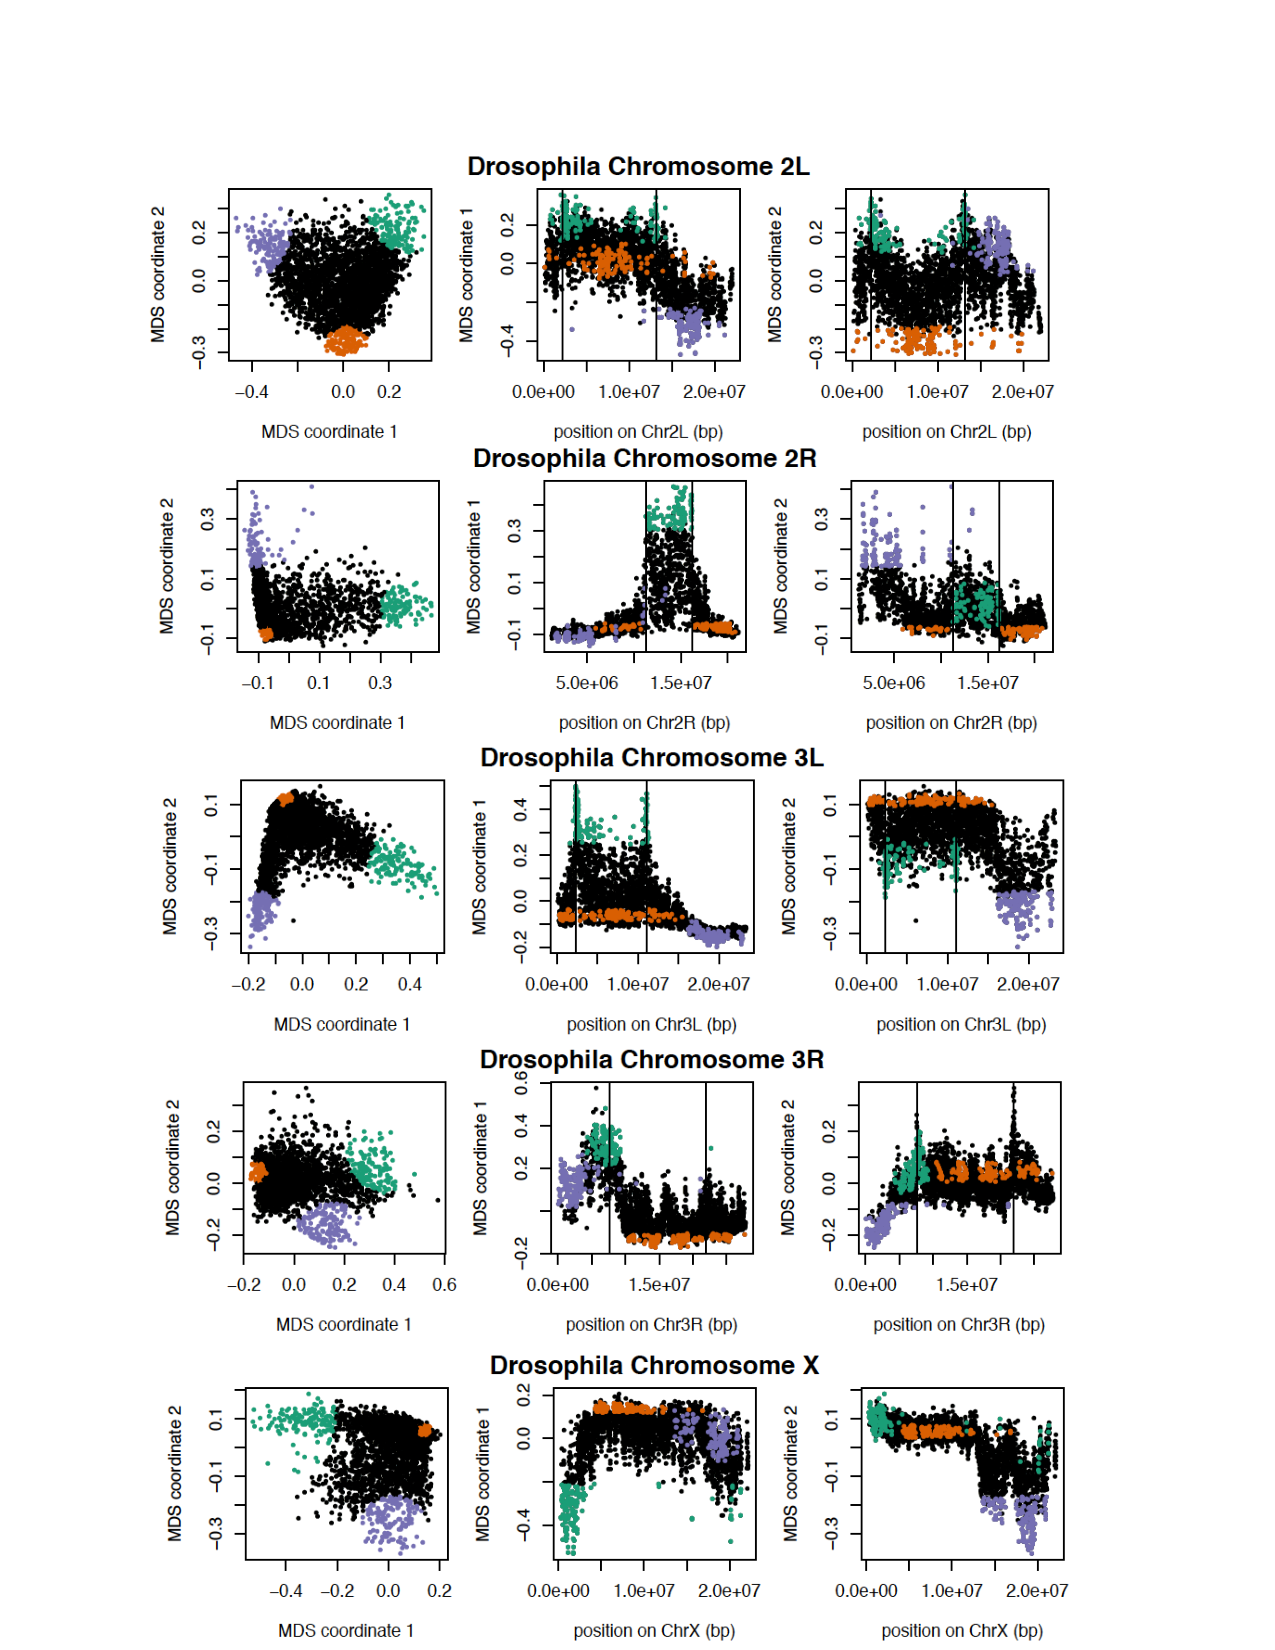
\includegraphics[width=0.9\textwidth]{Fig1}
    \end{center}
    \caption{
         Variation in structure for windows on chromosome arms 2L, 2R, 3L, 3R and X. 
         Each represents a window: the first column shows the MDS visualization of relationships between windows. 
         The second and third columns show the position (midpoint) of each window against the first and second MDS coordinates, respectively. 
         Rows show results from different chromosome arms, from top to bottom: Chr2L, Chr2R, Chr3L, Chr3R, ChrX. 
         Colors are consistent for plots in each row. 
         Vertical black lines show the breakpoints of known polymorphic inversions for Chr2L, Chr2R, Chr3L, Chr3R (from top to down: In(2L)t, In(2R)NS, In(3L)OK, In(3R)K).
         \label{fig:mds_chr2L}
    }
\end{figure}


To investigate these extremes, we pick a window for each extreme, 
and take out the 5\% of windows that are closest to it in the MDS coordinates, 
then combine those windows for each extreme and apply PCA on the corresponding sections of genome. 
We can see in Figure \ref{fig:pca_chr2L} the obvious difference between their PCA plots. 

\begin{figure}
    \begin{center}
       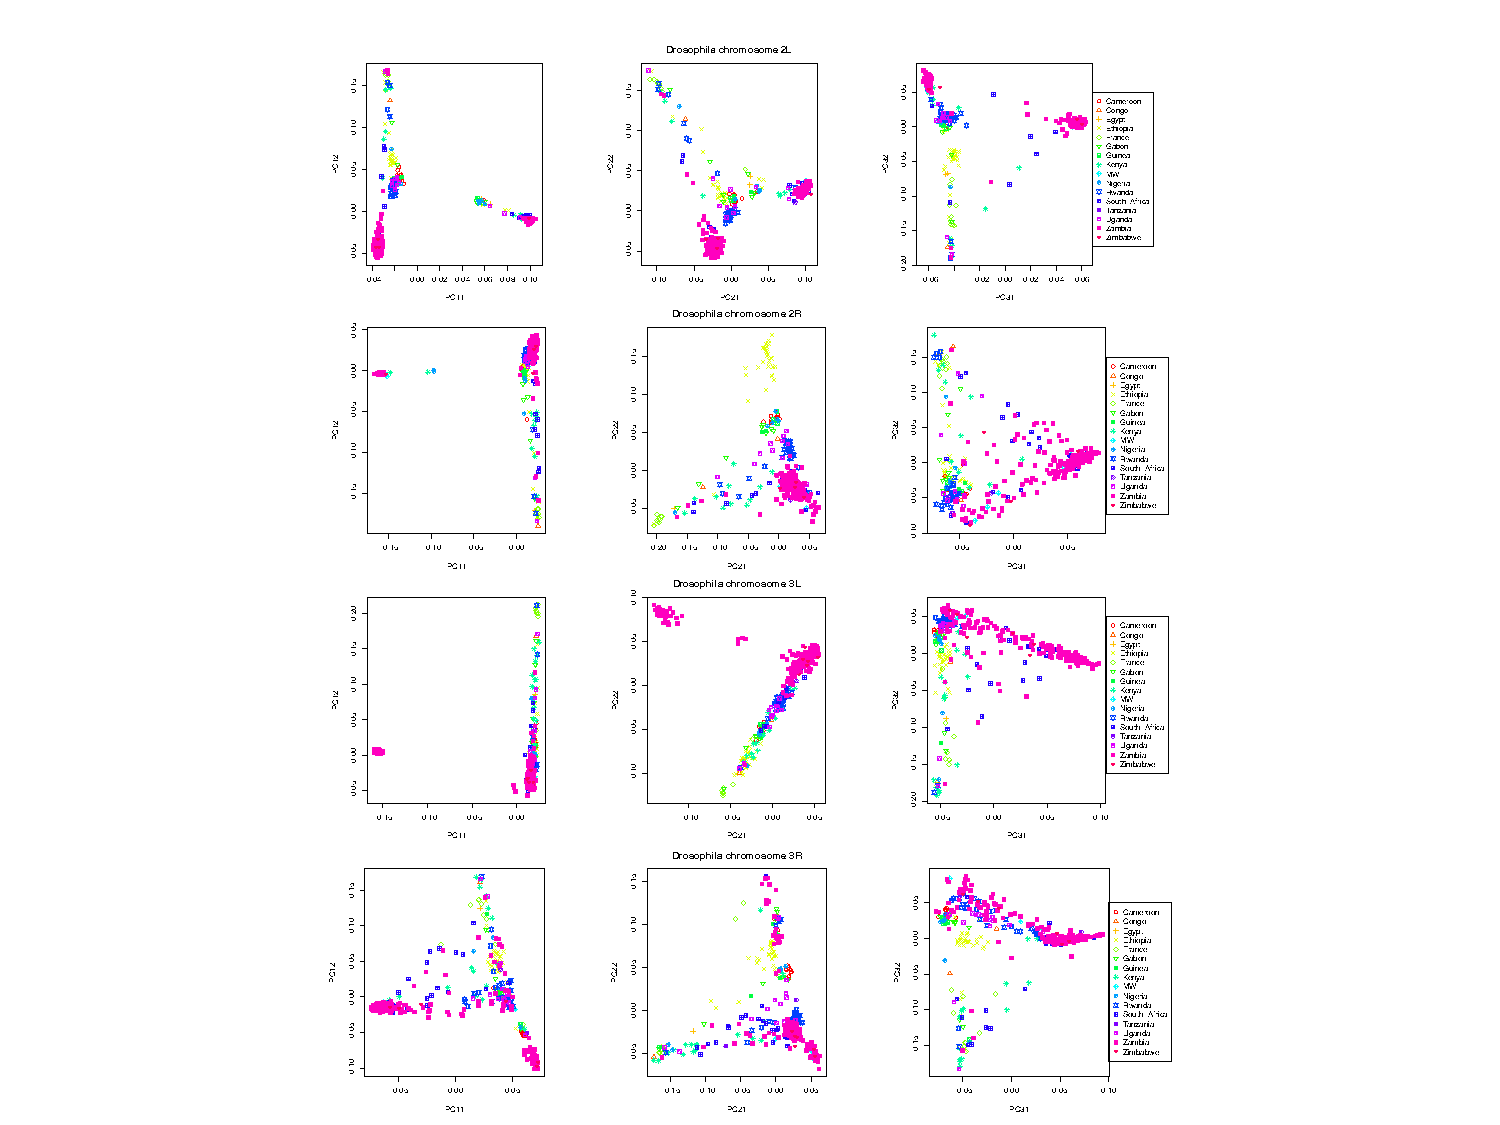
\includegraphics[width=0.9\textwidth]{Fig2}
    \end{center}
    \caption{      
        PCA plots for the three sets of genomic windows colored in Figure \ref{fig:mds_chr2L}. 
        Each point represents a sample. 
        The plots are plotting the second principal components against the first principal components. 
        The first column shows the windows colored green in Figure 1; the second column shows orange windows; and third shows purple windows.
         \label{fig:pca_chr2L}
    }
\end{figure}


There's a large inversion on Chr2L in that is polymorphic in these samples, In(2L)t \citep{corbett2012population}. We recolored the PCA plots in Figure \ref{fig:pca_chr2L} by the orientation of the inversion for each sample. Figure \ref{fig:color_inver}
Two regions of similar, extreme population structure (green in Figure \ref{fig:mds_chr2L}) are found around inversion breakpoints, 
and the other two extremes occur in the center of the inversion and between the inversion and centromere.
The corresponding PCA plots show that locally, population structure is mostly determined by which orientation of the inversion each sample has.
Similar results are found in other chromosome arms that have known polymorphic inversions (Chr2R, Chr3L, Chr3R) in \textit{Drosophila}. 
Other known polymorphic inversions are like In(3L)P on Chr3L, In(3R)Mo and  In(3R)P on Chr3R. 
In(3L)P and In(3R)Mo are just a few in our samples, thus we don't see the significant influence of population structure of them. 
The situation of Chr3R is a little complicated. The coexisting inversions make the MDS visualiazation of it more difficult to pick the extremes.
For the extremes we picked in Figure \ref{fig:mds_chr2L}, In(3R)K could best explain the PCA clustering result, 
while picking other windows as extremes might show that In(3R)P explain the PCA clustering result.

\begin{figure}
    \begin{center}
       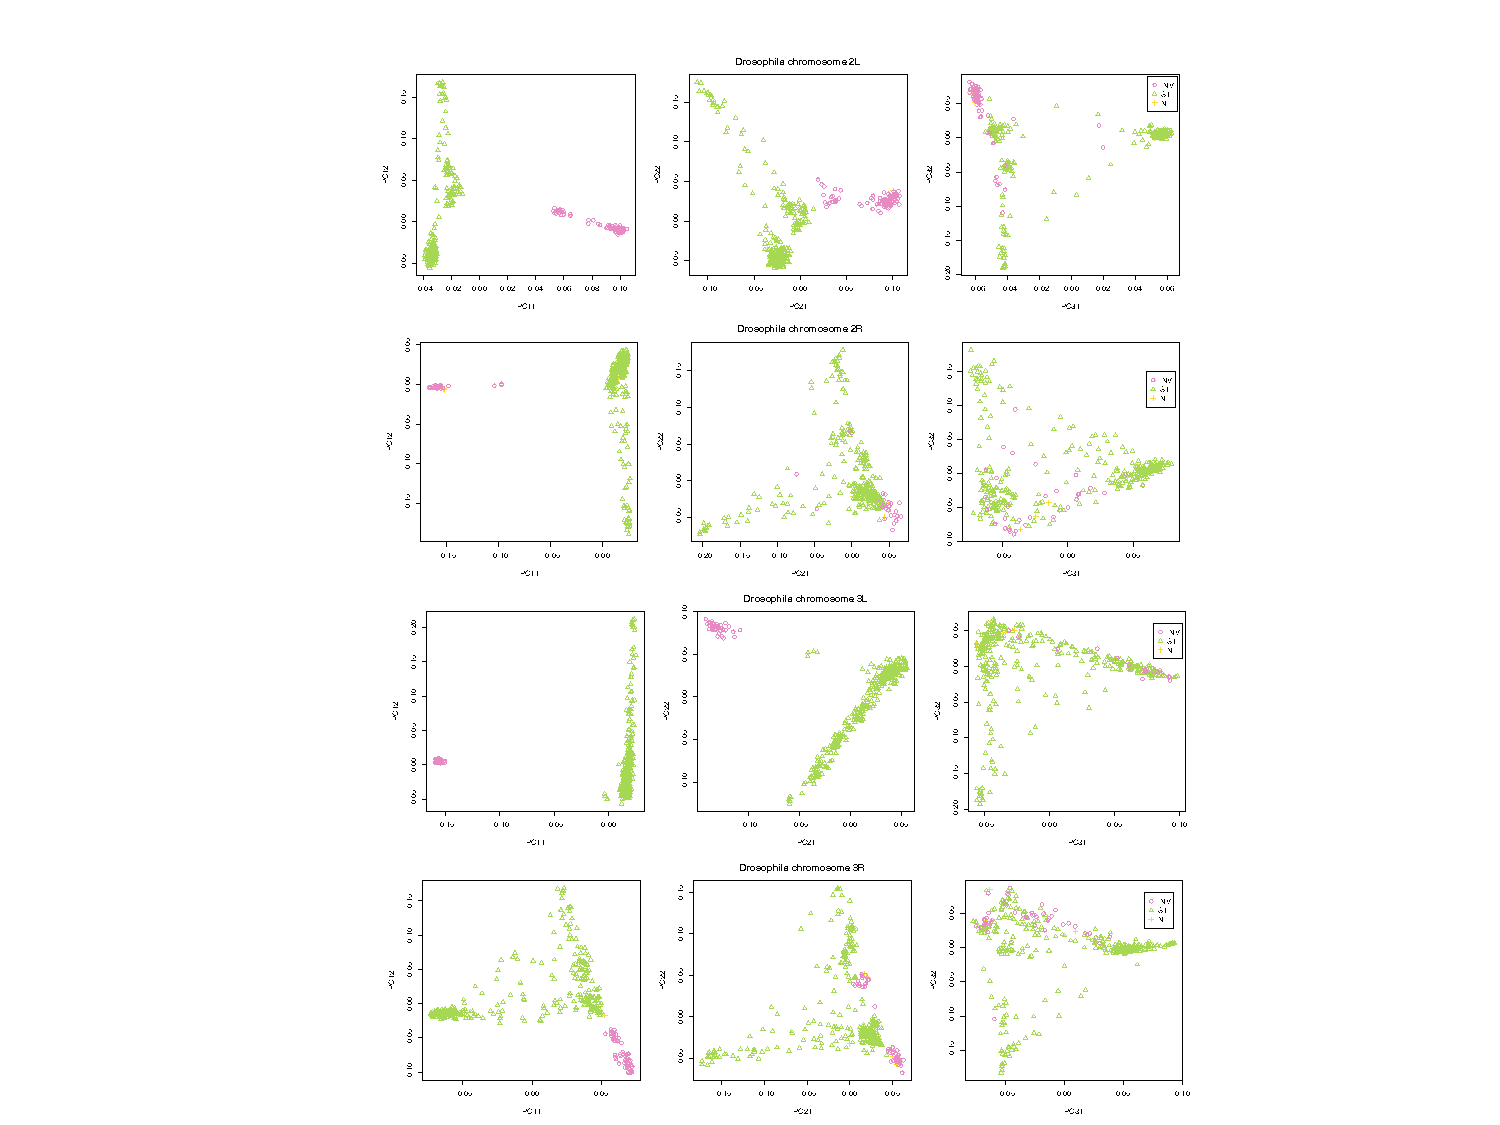
\includegraphics[width=0.9\textwidth]{Fig3}
    \end{center}
    \caption{
         As in Figure 2, except that samples are colored by orientation of the corresponding polymorphic inversion, In(2L)t, In(2R)NS, In(3L)OK and In(3R)K. (Data from \citet{lack2015drosophila}.
        \label{fig:color_inver}
    }
\end{figure}

\subsection{Human}
We ran our method separately on all 22 human autosomes. 
For instance, the eleven windows that are outliers in the first MDS coordinate of chromosome 8 (Figure \ref{fig:mds_human}b) coincide with the position of known polymorphic inversions on 8p23. 
Similar results are found in other chromosomes that have known inversions (eg. Chromosome 15, Chromosome 17).
We found that the primary axis of variation in population structure differentiated only one or a few windows on each chromosome, 
unlike the countinous variation in population structure we see in Drosophila.
Other chromosomes showed similar results around predicted inversions: PCA might provide an additional way to identify inversions \citep{ma2012investigation}.

When we run the method on all 22 autosomes together, the outlying signal of chromosome 8 is still visible. (See supplementary for all 22 autosomes)

\begin{figure}
    \begin{center}
       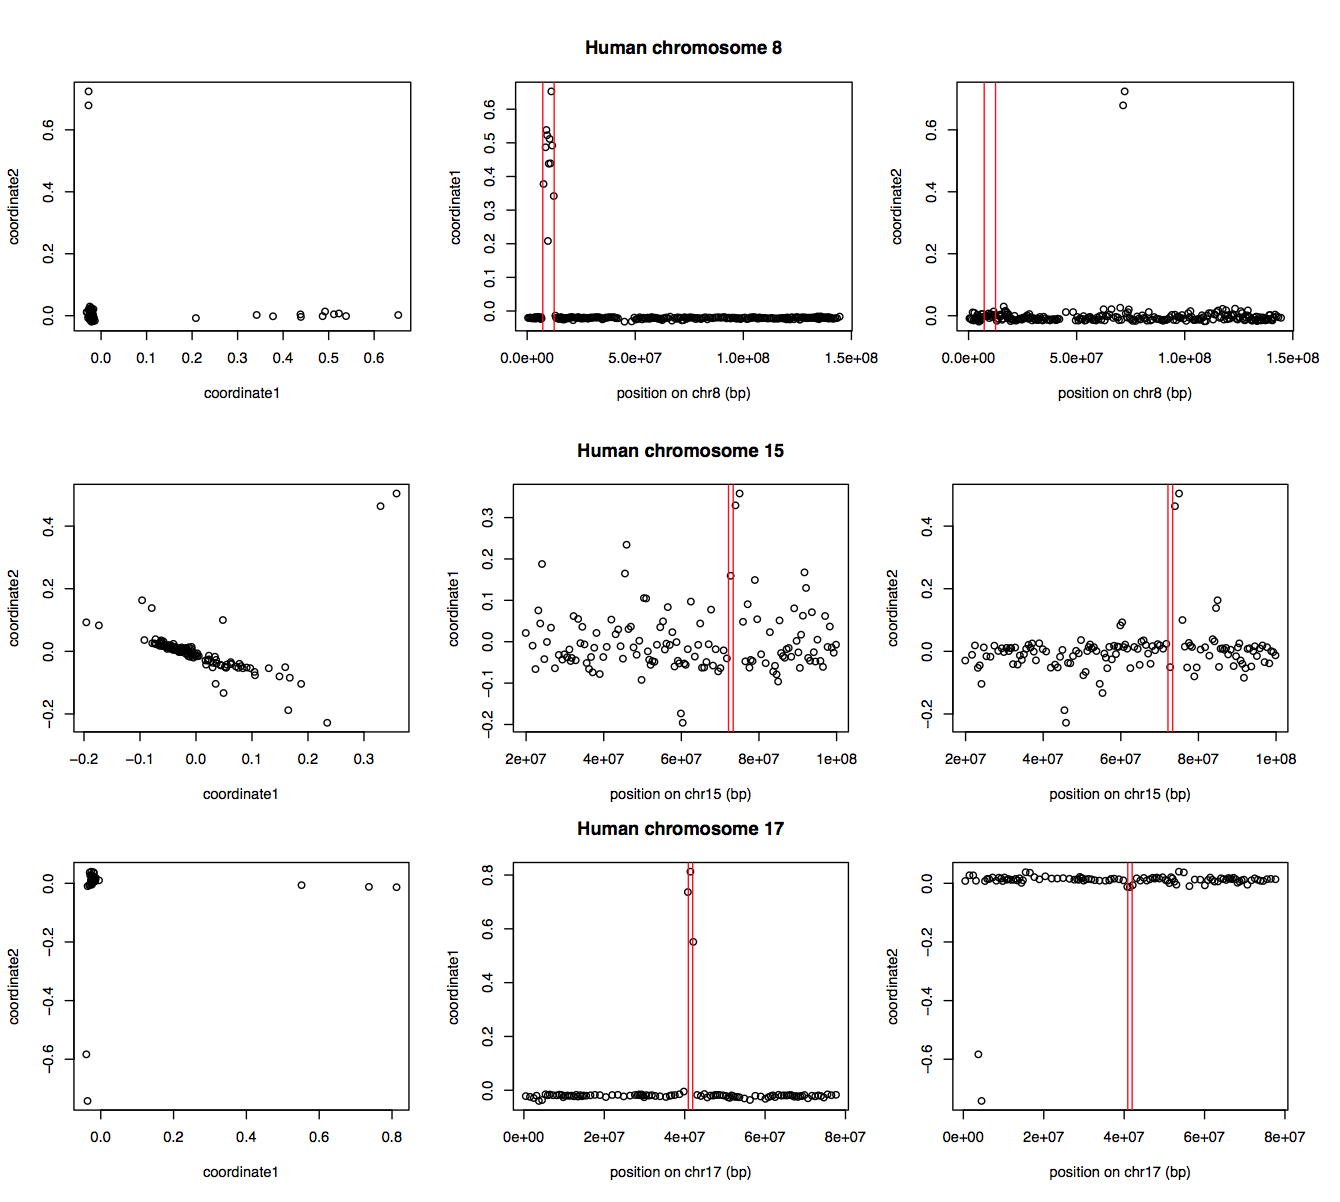
\includegraphics[width=0.9\textwidth]{Fig4_temp}
    \end{center}
    \caption{
         Variation in structure between windows on human chromosomes 8, 15, and 17. 
         Each point in the plot represents a window.
         The first column shows the MDS visualization of relationships between windows;
         the second and third columns show the two MDS coordinates of each window against its position (midpoint) along the chromosome. 
         Rows, from top to bottom show chromosomes 8, 15, and 17. 
         The vertical red lines show the breakpoints of the known inversions \citep{antonacci2009characterization}.
        \label{fig:mds_human}
    }
\end{figure}


\subsection{\textit{Medicago truncatula}}
We ran our method on all 8 chromosomes of \textit{Medicago truncatula} seperately 
and found the correlation between each MDS plot and gene density along the genome in all 8 chromosomes. 
This consistency implies that the factor driving the population structure for each chromosome might be the same, for example, background selection.
So we ran all chromosomes together, that is, calculating the pairwise distance for all the windows along 8 chromosomes,
and then get the MDS coordinates for each chromosome by locating the whole MDS coordinates.
\plr{The results looked different than the other two species, with much less pronounced peaks...}  
We computed gene density near each window using gene models in Mt4.0 JBrowse \citep{tang2014improved}. 
The first MDS coordinate value is negatively correlated to the gene count for each window (Figure \ref{fig:mds_gene_count}).
We found the position of the peak for each MDS plot has a coincidence with the position of heterochromatic regions. 
This means that population structure in the windows located in heterochromatin tends to have higher similarity, since those windows are closer in MDS plots.
Biologically, heterochromatic regions have lower gene density and may be less subject to selection \citep{kulikova2001integration,paape2013selection}. 
Besides, we found the PCA plots are quite consistent for the peaks that more clustering away from the heterochromatic regions, 
while the PCA plots are barely consistent for the peaks that more clustering around heterochromatic regions for the 8 chromosomes.
Unlike in the human and Drosophila genomes, in \textit{Medicago truncatula}, major variation in population structure is likely due to linked selection. 

\begin{figure}
    \begin{center}
       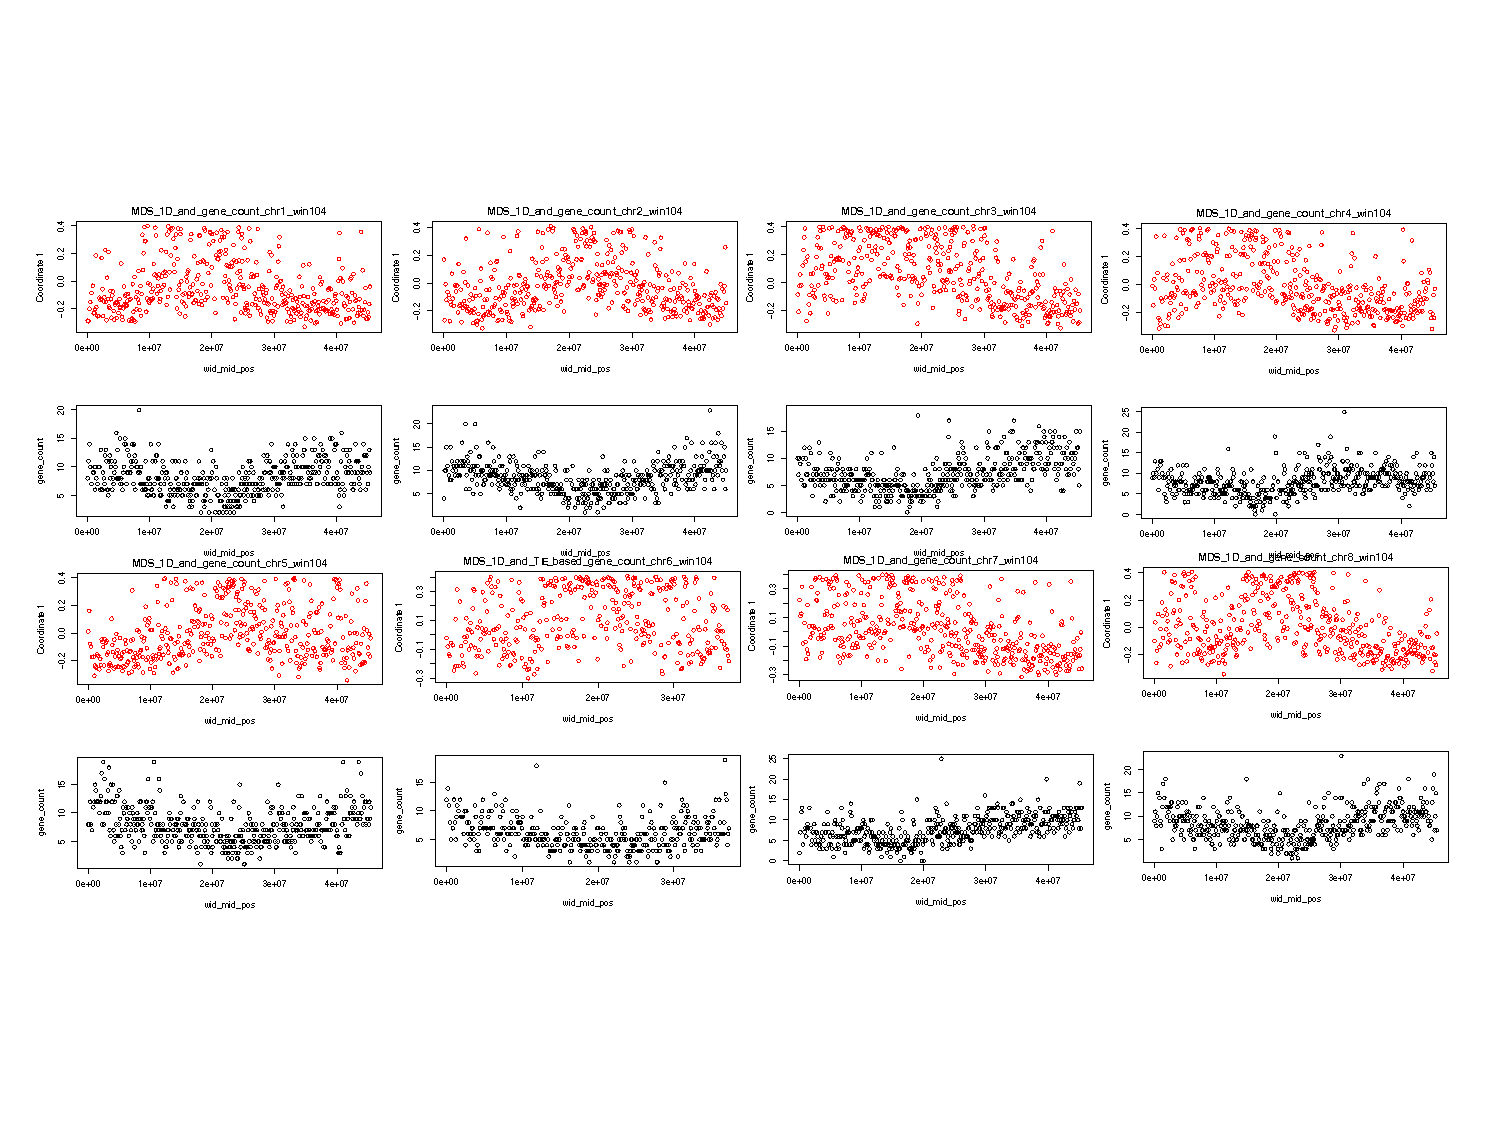
\includegraphics[width=0.7\textwidth]{fig5}
    \end{center}
    \caption{
         MDS results and gene density for the \textit{Medicago} genome (chromosome 1-8). 
         For each chromosome, the red plot above is first coordinate of MDS against the middle position of each window along each chromosome. 
         The black plot below is gene count for each window against the position of each window.
         \label{fig:mds_medicago}
    }
\end{figure}

\begin{figure}
    \begin{center}
       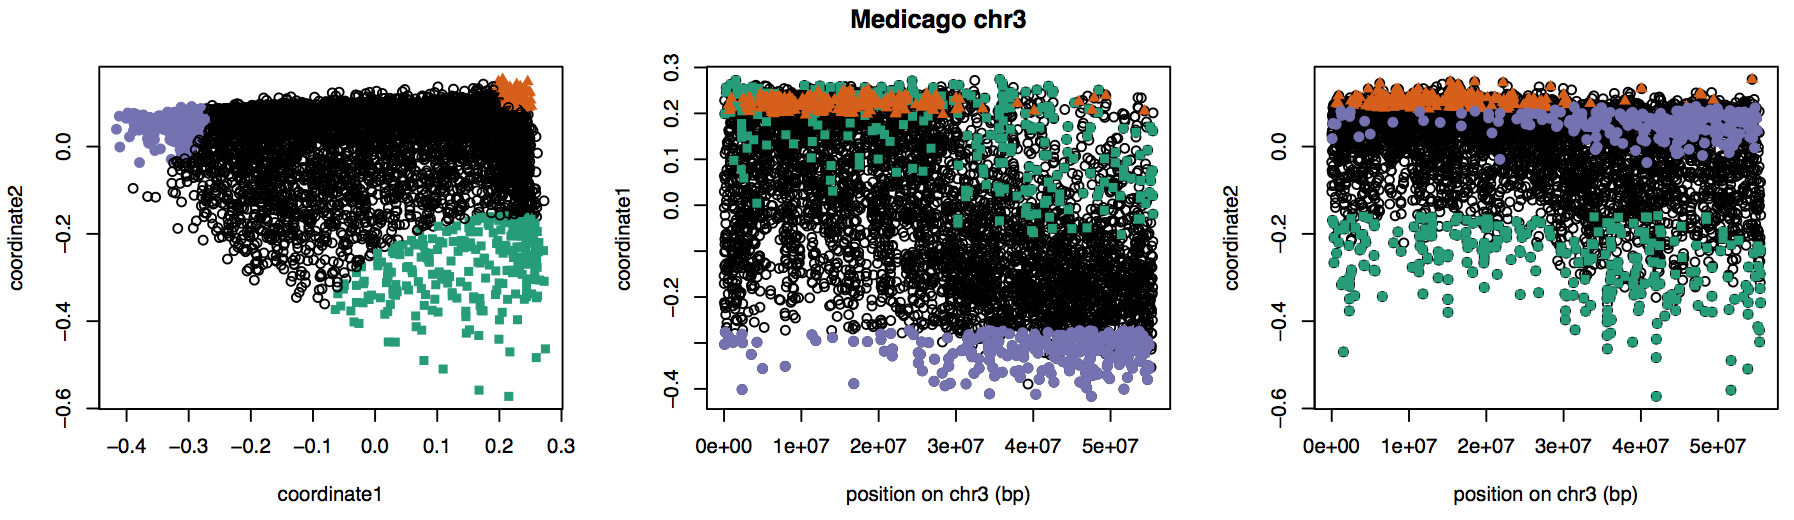
\includegraphics[width=0.9\textwidth]{medicago_mds}
    \end{center}
    \caption{
     MDS visualization for Medicago chromosome 3. Each point in the plot stands for a window (length 1000 SNPs).
       \label{fig:mds12_medicago}
    }
\end{figure}

\begin{figure}
    \begin{center}
       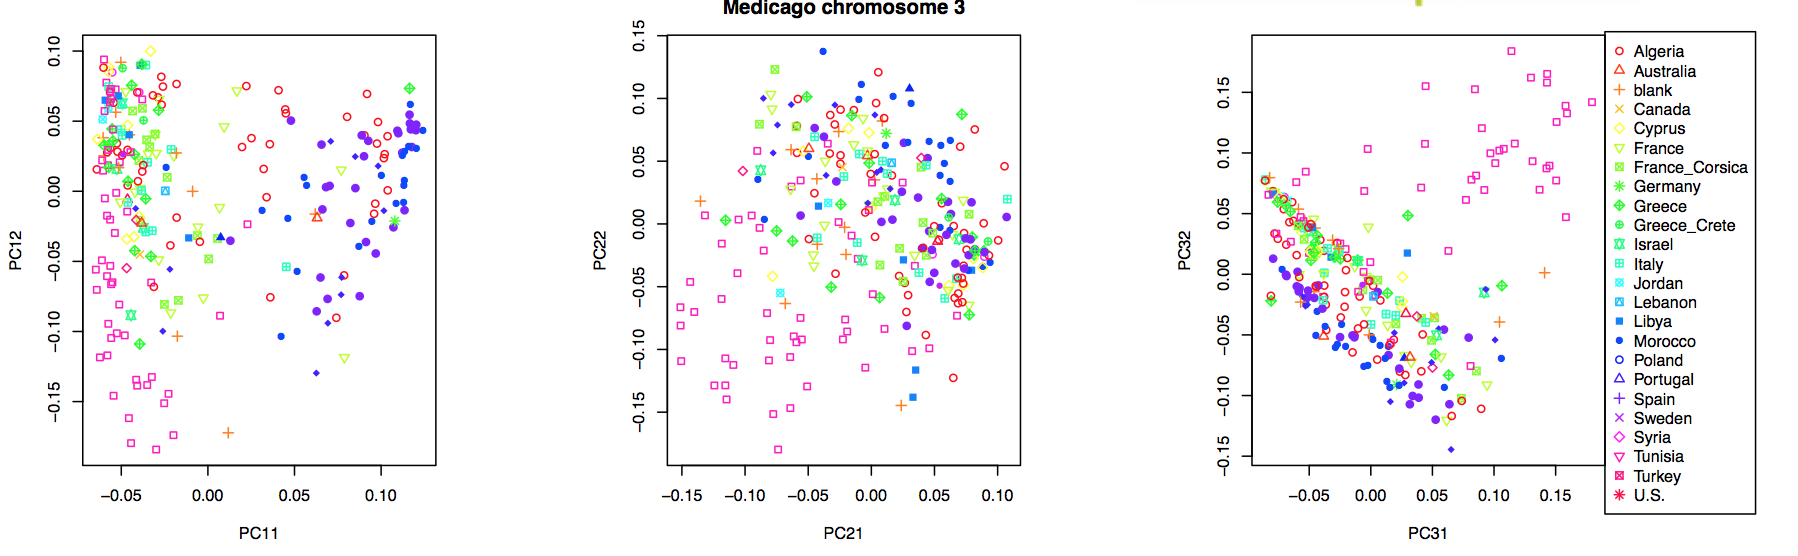
\includegraphics[width=0.9\textwidth]{medicago_peaks_pca}
    \end{center}
    \caption{
        PCA plots for the three sets of genomic windows colored separately in Figure \ref{fig:mds12_medicago}. 
        From left to right, the windows colored green, orange, and purple. Each point corresponds to a sample, colored by origin.
        \label{fig:pca_medicago}
    }
\end{figure}


\begin{figure}
    \begin{center}
       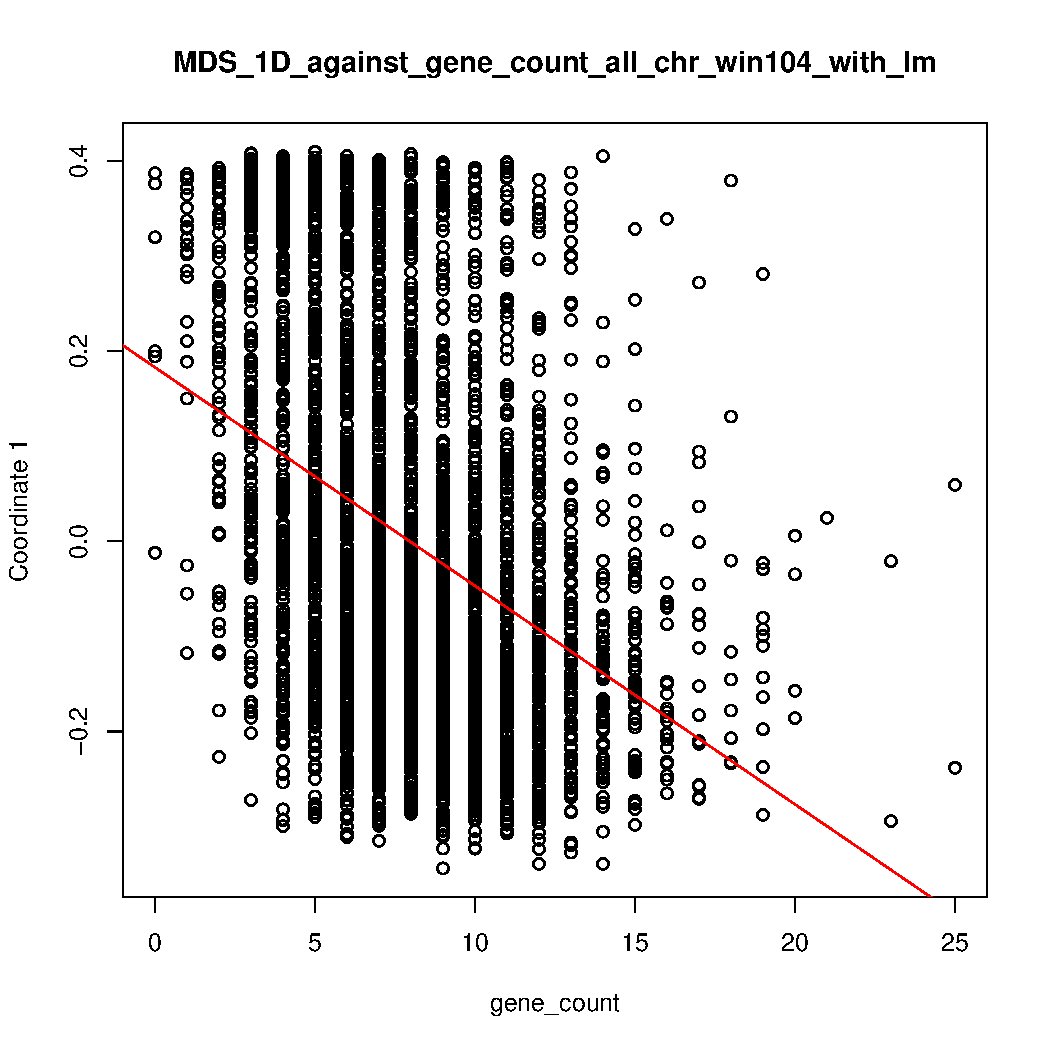
\includegraphics[width=0.9\textwidth]{Fig6_MDS_1D_against_gene_count_all_chr_win104_with_lm}
    \end{center}
    \caption{
        First MDS coordinate against gene density for all 8 chromosomes. 
        The first MDS coordinate is significantly correlated with gene count (r=0.146, p=$2.2\times 10^{-16}$). 
        (See supplementary for each single chromosome's MDS result against gene count for \textit{Medicago})
        \label{fig:mds_gene_count}
    }
\end{figure}

%%%%%%% %%%%%%%%%
\section{Discussion}

(sentence about how we found variation in pop structure)

With growing appreciation of the heterogeneous effects of selection across the genome,
especially the importance of adaptive introgression, hybrid speciation \citep{tomato,mosquito,introgression_review},
local adaptation \citep{local_adapt_review},
and inversion polymorphisms \citep{mosquito,kirkpatrick_inversions},
local PCA may prove to be a useful exploratory tool to discover important genomic features.
It is unclear whether the technique will be useful on reduced representation genotyping datasets 
due to marker density and issues with missing data --
our investigations with one such dataset were inconclusive --
but even low coverage, whole-genome sequence is very promising.


\paragraph{Confounding in GWAS}
So-called cryptic relatedness between samples
has been one of the major sources of confounding in genome-wide association studies (GWAS)
and so methods must account for it by modeling population structure or kinship \citep{gwas_confounding_review,mixed_models}.
Since population structure is not constant along the genome,
this could in principle lead to an inflation of false positives parts of the genome
with stronger population structure than the genome-wide average.
Fortunately, in our human dataset this does not seem likely to have a strong effect:
most variation is due to small, independent regions, possibly primarily inversions,
and so may not have a major effect on GWAS.
In the other species we examined, particularly \textit{Drosophila melanogaster},
treating population structure as a single quantity could be severely misleading.


\paragraph{Parameter choices}
There are several choices in the method that may affect the results.
As with whole-genome PCA,
the choice of samples is important,
as variation not strongly represented in the sample will not be discovered.
The effects of strongly imbalanced sampling schemes are often corrected by dropping samples in overrepresented groups;
but downweighting may be a better option that does not discard data.
Next, the choice of window size may be important,
although in our applications results were not sensitive to this,
indicating that the limit of resolution was smaller than the scale on which patterns of kinship varies along the genome.
Finally, which collections of genomic regions are compared to each other (steps 3 and 4 in figure \ref{fig:diagram}),
along with the method used to discover common structure,
will affect results.
We used MDS, applied to either each chromosome separately or to the entire genome;
for instance, human inversions are clearly visible as outliers when compared to the rest of their chromosome,
but genome-wide, their signal is obscured by the numerous other signals of comparable strength.

Besides window length, there is also the question of how to choose windows.
In these applications we have used nonoverlapping windows with equal numbers of polymorphic sites.
Alternatively, windows could be chosen to have equal length in genetic distance,
so that each would have roughly the same amount of phylogenetic information.
However, given the insensitivity of our results to window length,
this seems unlikely to give different results.
\plr{If we check: We did not have this choice to have a substantial effect on results.}

More generally, there are many possible methods to discover common structure in different parts of the genome.
The methods we chose discovered strong biological signal of different types in three datasets;
but it is possible that other methods for measuring dissimilarity between windows' covariance matrices
or for summarizing the matrix of pairwise distances between windows
would lead to different insights.
Minor points we have not explored include how to decide how many PCs to use in approximating structure of each window
(equations XX),
how many MDS coordinates to use when describing the distance matrix between windows,
or how to choose interesting regions of the genome when the MDS plot is not triangular.
These are all part of more general techniques in dimension reduction and high-dimensional data visualization;
we encourage the user to experiment.


\paragraph{Chromosomal inversions}
A major driver of variation in population structure in two datasets we examined are inversions.
This may be common,
but the example of \textit{Medicago truncatula} shows that polymorphic inversions are not ubiquitous.
PCA has been proposed as a method for discovering inversions \citep{ma_identify_inversions};
However, the signal left by inversions likely cannot be distinguished from long haplotypes under balancing selection 
or simply regions of reduced recombination.
However, in many applications, inversions are a nuisance.
For instance, SMARTPCA \citep{smartpca} reduces their effect on PCA plots
by regressing out the effect of linked SNPs on each other.
It would be interesting to see if smoehow removing the effects of inversions in the \textit{Drosophila melanogaster} or human datasets
would produce a pattern similar to that seen in \textit{Medicago truncatula}.

\plr{Check if I've missed anything, then remove these?}

\subsection{Future work}
1. For human and Drosophila, we want to eliminate the regions under known inversions and check the variation of population structure for the remaining part by removing those sections. We try to check whether they will give similar results as in \textit{Medicago truncatula}, that is whether the variation is closely related to heterochromatin or gene density.

\noindent 2. Uneven sampling has a strong influence on PCA projections \citep{mcvean2009genealogical}. 
Our human data, POPRES, is unevenly sampled including 346 African-Americas, 73 Asians, 359 Indian Asians and 3187 Europeans. 
First, we'll try sub-sampling Europeans to balance the population size for the 4 population and repeat the process on the resampled data. 
Second, we'll try to apply the whole process on only European samples to see the genetic variation inside European samples. 
Third, we want to try different scheme of adding a weighting matrix to the covariance matrix of genotype data, thus to the reduce the influence of uneven sampling.

\noindent 3. Since regions that have low recombination rate tend to have similar PCs, we'll try cutting the chromosomes into windows with same distance in genetic map instead of same SNP numbers.

\noindent 4. Euclidean distance between the contracted matrix based on PCs is one measure of the similarity for window's population structure.
We want to try other methods of distance between windows, for example, we used the distance for PCs to reduce noise, however the distance between covariance matrixes of genotype matrix might also be informative.

\noindent 5. Although the first two coordinates contains the main part of information, we'd like to see the information contained in higher PCs (e.g. the third PC, the forth PC), and higher dimension of MDS.

\bibliographystyle{plainnat}
\bibliography{references}  
\end{document}  
